\chapter{Introduction}
\label{ch:introduction}
\minitoc

\section{Learning from graph-structured data}
\label{sec:motivation}

Data in machine learning often comes in a few familiar forms.
Most datasets are tabular: a table of rows and columns in
which each row is an independent example described by the same fixed set of
features. Other data is organized as images, that is, grids of pixels, or as
sequences such as text and audio, whose elements follow one another in a specific order. 
What these forms share is regularity: each has a fixed,
well-defined structure that repeats across every example.

Many real-world systems do not fit any of these shapes. A molecule
is a set of atoms connected by chemical bonds, and neither the
number of atoms nor the way they are connected is the same from one molecule to
the next. A social network is a set of people connected by relationships, where
each person may be linked to a different number of others. A citation network is
a set of papers that reference one another, each citing a different set of
others. These are not tables, images, or sequences; they are networks of
entities and the relations between them (Figure~\ref{fig:graph-structured-data}).
Data of this kind is naturally described by a \textit{graph}: a set of entities,
called \textit{nodes}, together with a set of connections between them, called
\textit{edges}. Both nodes and edges can carry their own data. For example, in a molecule,
each node is an atom labeled with its element (such as carbon, hydrogen, or oxygen),
and each edge is a bond of a particular type (such as single, double, or triple); in
a social network, the nodes are people and the edges are the relationships among
them.

\begin{figure*}[t]
  \centering
  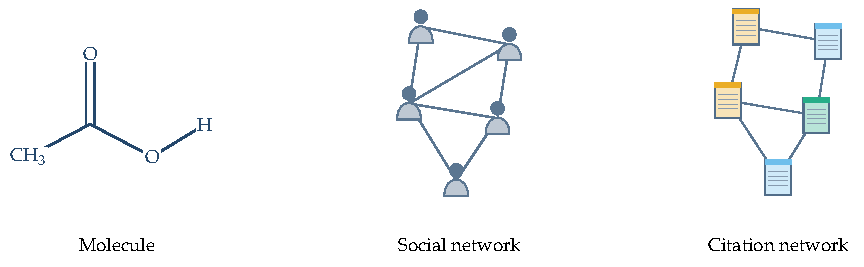
\includegraphics[width=\textwidth]{graph-structured-data}
  \caption[Examples of graph-structured data.]{%
    Three domains represented as graphs. A molecule, whose nodes are atoms
    labeled by their element and whose edges are bonds (single or double); a
    social network, whose nodes are people and whose edges are relationships;
    and a citation network, whose nodes are papers (colored by topic) and whose
    edges are citations between them. In each case the entities and their
    connections, rather than a table, grid, or sequence, define the structure of the data.
  }
  \label{fig:graph-structured-data}
\end{figure*}

Rather than treating a domain as a collection of isolated data points, it can be
described in terms of entities and the relationships among them, which means
there is an underlying graph whose structure ties those entities together. Seen
this way, the graph is not merely one possible encoding of a molecule or a
social network but a faithful representation: it records exactly
which entities exist and how they relate, without forcing the data into a shape
it does not have. A wide range of domains exhibit this kind of relational
structure, and modeling them explicitly as graphs, rather than ignoring the
connections, can lead to better predictions~\cite[3.5pc]{battaglia2018}. Data
organized in this way is called \textit{graph-structured data}.

Most deep learning models are tailored to the regular structures
described above. Graphs are harder to work with. 
They have no fixed size, since different graphs contain
different numbers of nodes. They have no fixed layout: a pixel in a grid has a
clear sense of place, with neighbors above, below, and to either side, whereas a
node in a graph has no such spatial arrangement and may be connected to any
number of others. And they have no natural ordering, with no first or last node
and no canonical point from which to read the rest.

The goal, then, is a model that takes a graph as input and produces
predictions about it, such as a label for each node, a connection between
two nodes, or a single label for the graph as a whole. This raises
the central question: how can a predictive model -- concretely, a neural
network -- be designed to operate directly on a graph, respecting its variable
size and its lack of order instead of discarding them? Neural networks built for
this purpose are called \textit{Graph Neural Networks},
hereafter abbreviated as GNNs~\cite{hamilton2020}.

\section{Objectives and scope}
\label{sec:objectives-scope}

The general objective of this work is to provide a self-contained
reference on GNNs for homogeneous graphs under the \textit{message-passing}
framework: a single document that assembles the theory that motivates and defines
these models, presents representative architectures, and 
evaluates them through reproducible implementations.

Specifically, the work aims to:

\begin{itemize}
  \item establish the foundations that motivate GNNs: how graphs represent
        relational data, why standard neural networks cannot learn from it
        directly, and the inductive biases a model on graphs must respect;
  \item develop the message-passing framework as the unifying formulation from
        which GNN architectures are derived;
  \item present representative architectures for the three standard learning
        tasks on graphs: the Graph Convolutional Network (GCN)~\cite[-12pc]{kipf2017}
        for node classification, the Graph Autoencoder (GAE)~\cite[-7.5pc]{kipf2016} for
        link prediction, and the Graph Isomorphism Network (GIN)~\cite[-4.5pc]{xu2019}
        for graph classification;
  \item implement the three architectures on standard benchmark datasets
        (Cora, Amazon Computers, and NCI1)~\cite[-2.2pc]{sen2008,shchur2018,wale2008}
        using PyTorch Geometric, ensure reproducibility, and evaluate each
        against a multilayer perceptron baseline;
  \item examine the principal limitations of GNNs under this framework,
        including oversmoothing~\cite[0.6pc]{li2018},
        oversquashing~\cite[0.5pc]{alon2021}, heterophily~\cite[0.5pc]{zhu2020}, and the
        ceiling on their expressive power~\cite[0.5pc]{xu2019}.
\end{itemize}

The contribution of this work lies not in the material itself, which is
documented in the literature cited throughout, but in the arrangement of that
material and in the experimental analysis built on it. The theory is presented
under a single notation, so that architectures introduced in separate papers,
each with its own conventions, appear as instances of one general formulation
rather than as unrelated constructions. Each formal object is paired with an
executable counterpart, so that a derivation and the code that realizes it can
be read against each other. And the multilayer perceptron, the model whose
failure on graphs motivates the framework, is recovered within that same
framework as what message passing reduces to on a graph with no edges.

This last point defines the role of the experiments: the multilayer perceptron
is a baseline that receives the data of each node but nothing about its
connections. Each architecture is compared against it under a common protocol
and over runs with different seeds, and the comparison is analyzed rather than
only reported.

The graphs considered in this work are treated mainly as
undirected, meaning their connections carry no direction, and
simple, meaning that at most one connection joins any pair of nodes and
that no node is connected to itself. This choice reflects simplicity rather than a limitation 
of the framework: message passing has enough design space to accommodate directed graphs,
self-loops (a node connected to itself), and even
multigraphs (more than one connection between the same pair of nodes).

The graphs considered in this work are also homogeneous: they contain a single kind of node
and a single kind of connection. This restriction is deliberate. The
homogeneous setting is where the message-passing framework is most directly
understood, and it is the foundation on which more elaborate models are built,
including heterogeneous graphs, which carry several kinds of nodes and
connections and require machinery beyond the scope of this work.

The concepts introduced here are defined formally throughout the remainder of the document.

\section{Structure of the document}
\label{sec:document-structure}

This introduction has set out the motivation, objectives, and scope of the
work, together with what it contributes.
The remainder of the document is organized as follows.

The first chapters establish the foundations. Chapter~\ref{ch:applications}
surveys the tasks that graph learning addresses at the node, edge, and graph
level, together with practical applications that motivate the rest of the work.
Chapter~\ref{ch:graph-theory} establishes the formal definitions and notation
for graphs used throughout. Chapter~\ref{ch:nn-limitations} reviews the
multilayer perceptron and shows why standard neural networks are ill-suited to
relational data. Chapter~\ref{ch:inductive-bias} develops the notion of
inductive bias and the permutation invariance and equivariance that any graph
layer must satisfy.

Chapter~\ref{ch:message-passing} builds on these foundations to derive the
message-passing framework: the message, aggregation, and update functions, the
receptive field that successive layers induce, the expressive power of the
resulting models, and the architectural design space it enables.

Chapter~\ref{ch:architectures} presents three representative architectures
within this framework: GCN for node classification, GAE for link prediction,
and GIN for graph classification. Chapter~\ref{ch:implementations} turns to
practice, providing reproducible implementations of these architectures on the
Cora, Amazon Computers, and NCI1 benchmarks in PyTorch Geometric, comparing each
against a multilayer perceptron, with the code available
in a companion repository~\cite{macias2026}.

Chapter~\ref{ch:limitations} examines the limitations of GNNs under the
message-passing framework, and Chapter~\ref{ch:conclusions} synthesizes the
work and outlines directions for future research.

